\chapter{Preliminaries and Subproblems}
\label{chapter:2}

%\section{Path Selection of Mobile elements}

It is known that controlled MULEs can increase a WSN's lifetime by enabling sensor nodes to save energy. But the problem of energy efficient data collection by MULEs depend on planning optimal paths and job schedules of MULEs. The problems are clubbed togather under the Data MULE scheduling problem~\cite{dms}. In general, achieving the goals of MULEs scheduling problem are 
hard, and consists of following components: 
\begin{enumerate}
  \item {\em Path selection}: determines the trajectory the data MULE 
    will follow.
\item {\em Speed control}: determine how the MULE will change the speed
  while moving along a trajectory. 
\item {\em Job scheduling}: determines the sensor from which a MULE collects data at each time point
\end{enumerate}
In this thesis our focus is only on path selection of the MULEs.

\section{Geometric Disc Covering and Location Nodes}

In the interest of collecting data from sensors in one hop, we propose to cover the sensor field with circular discs of radius equal to the range of the sensors. The centers of these will be locations where MULEs will pause to collect data from the sensors. For convinience in description, we will refer to these positions as \emph{location nodes}. At a location node, a MULE polls nearby sensors with the same transmission power as sensors, such that sensors that receive the polling messages can upload packets to the MULE within a single hop. Each sensor may be covered by more than one location nodes, but each sensor is associated with only one of these location nodes for data uploading to the MULE. Our path selection heuristic, proposed in Chapter~\ref{chap:steiner}, uses location nodes as the nodes of a graph embedded on the 2D plane, referred to as \emph{location graph}. Underlying assumptions in our approach are: (i) communication region of a sensor is approximated to a circular disc, (ii) all sensor have same communication range, and (ii) the range of the MULE is greater than that of any sensor. % (we assume all the sensors are identical in communication range). The centres of these discs are called \emph{location nodes}.

There are two types of geometric disc cover problems:

\begin{description}
\item[Geometric minimum disk cover (GMDC)] In this problem, a field of nodes is given, and the aim is to cover all the nodes with minimum number of discs (of given radius) possible. The centers of the discs can lie anywhere on the field.
\item[Geometric discreet unit disc cover (GDUDC)] In this problem, in addition to a field of nodes, a set of points $C$ is also given. The aim is to determine the smallest subset $C'$ of $C$, such that the discs placed at the points in $C'$ cover all the nodes in the field.
\end{description}

Though GDUDC was much more extensively explored compared to GMDC, we have 
used GMDC. Initially, we planned to get an intermediate solution of GMDC through some heuristic/Approximation Scheme, then apply techniques for GDUDC problem for a better solution. Due to our unclear understanding of the algorithm, however, we tried but failed to implement one solution~\cite{carmi} for GDUDC. Therefore, we relied on heuristics for find a disc covering.

Many heuristics and approximation schemes~\cite{shifting}, \cite{appScheme} have been proposed for GMDC. Any one of these can be possible candidates. We considered four main heuristics, here referred to as, Johnson's greedy set cover (JGRD), Greedy cover of sorted positions (GRD), Selection of smallest cover (SEL), Hexagonal tiling (HEX), and one approximation scheme know as Shifting strategy (SHFT) and carried out experiments for their efficacy in sample fields. 

%{\bf Comments: You need to give full form of each abbreviations first time you used them. There after abbreviations can be used.}

\subsection{Preliminaries}\label{subsec:prelim}

For convenience in subsequent description, we introduce certain preliminary
notations and concepts. Also, the "point" used here, can be a place holder for "sensor position", "sensor node" and "node" in subsequent description. Let $P$ be the set of points to be covered with discs of radius $R$, in the square field $F$. For any two $p_1, p_2 \in P$, there are two $c_1,c_2 \in F$ (called "crosses" for convinience) such that $p_1$ and $p_2$ will lie at the boundary of a disc of radius $R$ placed at either $c_1$ or $c_2$. We consider points $p_1$ and $p_2$ as covered (barely) by any of the two discs above. For any two points $p_1$ and $p_2$ such that distance between $p_1$ and $p_2$ is less than $2R$, there exist two crosses $c_1$ and $c_2$ ($c_1$ and $c_2$ are said to "involve" $p_1$ and $p_2$ for convinience). Let $C$ be the set of all possible crosses in the field $F$.

A set $S$ of disc centres such that they cover all the points in the field $F$ is called a solution of the GMDC problem in the field $F$. Let $S_1$ be such a solution. Then there exists a solution $S_2 \subset C$ such that $|S_1|=|S_2|$.

\subsection{Heuristics and the Approximation Scheme}

We focused on implementing four heuristics and one aproximation scheme to
obtain covering sensor fields. We provide a synopsis of these techniques
before discussing the results.

\paragraph*{OPT} 
This is an algorithm for the optimum solution, which uses brute-force to search for the minimum set cover in order to find the optimum solution. At first we create a table of the information regarding which cross (refer~\ref{subsec:prelim}) covers which of the sensors. These crosses act like the subsets of the set of all sensors containing the sensors they cover. Next, we find the minimum set cover using brute-force. Needless to say, the running time of this algorithm blows up very fast.

\paragraph*{HEX} 
In this heuristic~\cite{hex}, the sensor field is initially tiled with regular hexagons of sides equal to the radius of the discs to be used (see, figure~\ref{fig:hex}). A sensor is said to be covered by a hexagon, if it is closer to its center than the center of any other hexagon.

\begin{figure}
\centering
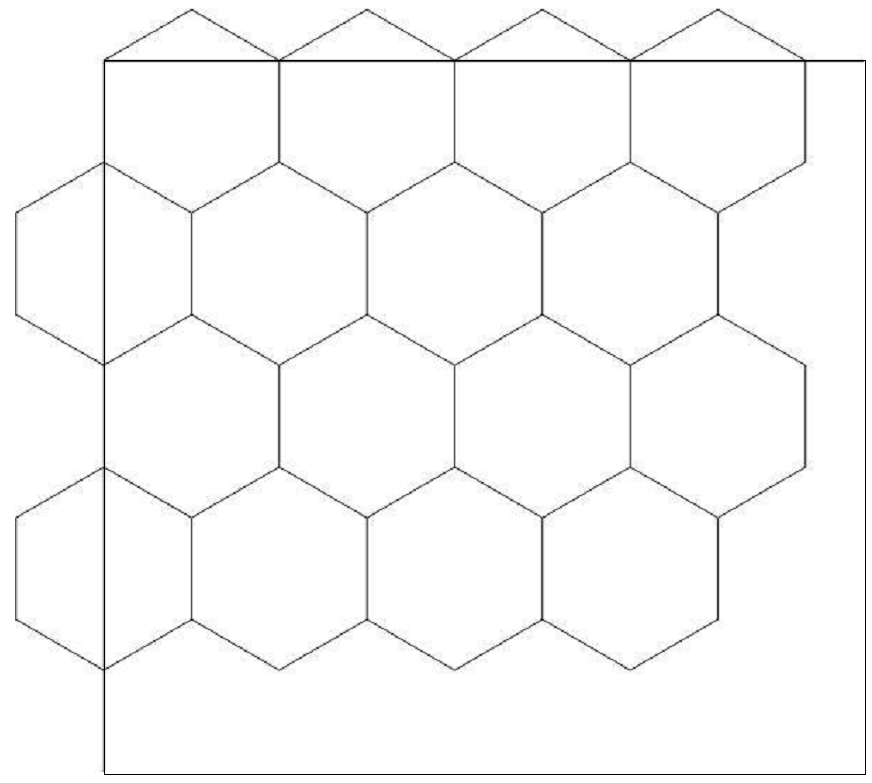
\includegraphics[width=8cm]{figures/hex.png}
\caption{Hexagonal tiling}\label{fig:hex}
\end{figure}

\paragraph*{JGRD} 
This is originally a set cover heuristic~\cite{jgreedy}. Consider the set $P$ as the target set to be achieved from the union of smaller subsets, and the discs centered at the crosses in $C$ represent the subsets of points covered by them. Our problem of MGDC then becomes a set cover problem. 
The reference~\cite{jgreedy} gives a greedy heuristic for this.

\paragraph*{GRD} 
(We have designed this heuristic, and we are not aware of any other work using it) Let the list of all sensor positions in the given field of sensor nodes be $L$. First sort $L$ according to their $(x,y)$ position co-ordinates (first by $x$ co-ordinate and then by $y$ co-ordinate). Starting from the first sensor node $p$ in the list, pick the disc which covers maximum number of uncovered sensor nodes and covers $p$ too. To do this, compute all the crosses in $C$ which involve $p$ (refer \ref{subsec:prelim} for "crosses" and "involving a node"). Place a disc of radius $R$ at each of the crosses, and choose the cross whose disc covers the most number of points. Choose the next uncovered sensor in $L$ and repeat the covering procedure, until all sensors are covered.

\paragraph*{SHFT} 
The shifting strategy is derived from~\cite{shifting}. This algorithm takes two input parameters: $l$ (shifting parameter, chosen later) and $D$ (diameter of discs to be used for covering). Let the field be a square of length $W$. First we divide the field into vertical strips of width $l \times D$, as shown in figure~\ref{fig:origStrip}. We do disc cover on these vertical strips (explained later) individually (treating them as separate fields. The union of the solutions of all the vertical strips is clearly a solution to the problem. This solution is assigned to $current\_solution$. Now, the whole partition of strips is shifted horizontally, away from the origin, by the amount of $D$ (as shown in figure \ref{fig:shiftStrip}). Again, all the strips are covered with discs (to be explained later how), and the union of the solutions of these shifted vertical strips another solution, assigned to $new\_solution$. If the size of $new\_solution$(the number of discs in the solution) is less than the size of $current\_solution$, the current solution now becomes $new\_solution$. We continue shifting the partition and measuring the solutions thus generated $l-1$ times.

To cover a strip of width $w$, we again apply the shifting strategy. We divide the strip into squares of side $w$ (and maybe a remainder rectangle, in case $W$ leaves a remainder upon dividing with $w$). To cover this sqaure (of size $w \times w$) with discs of diameter D, we use the strategy OPT described above. The shifting of this partition is done by the amount $D$ just like in the original field, and the smallest solution is chosen. The shifting parameter $l$ depends on the time constraint one has regarding the running time of this algorithm. It is chosen in such a way that the problem size in each sqaure (of size $w \times w$) is small enough for the OPT to run in required time constraint.

\begin{figure}[H]
\centering
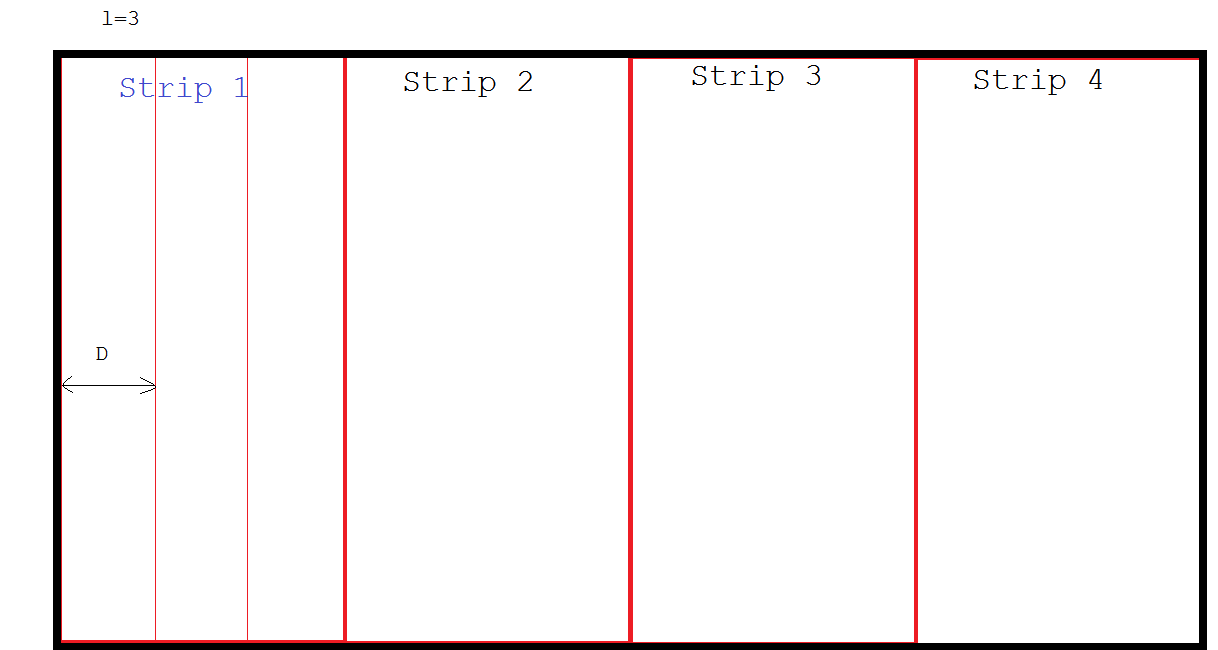
\includegraphics[width=15cm]{figures/beforeShift.png}
\caption{Original division of the field into vertical strips. $l$ is 3 here.} \label{fig:origStrip}

\end{figure}

\begin{figure}[H]
\centering
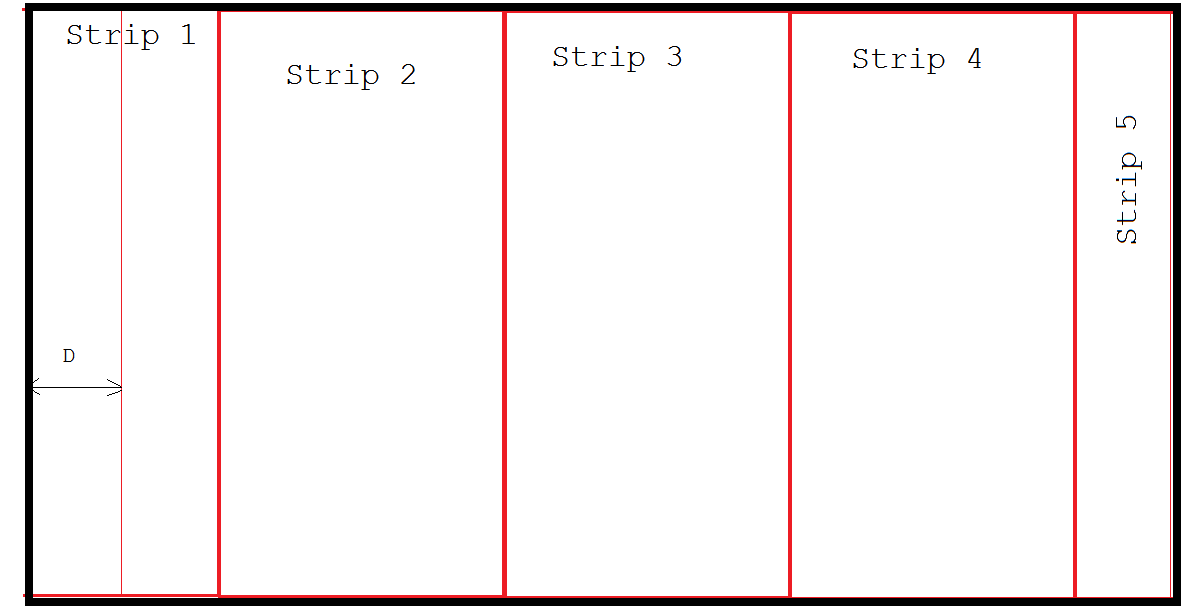
\includegraphics[width=15cm]{figures/afterShift.png}

\caption{After the shift right by the amount $D$}\label{fig:shiftStrip}

\end{figure}

\paragraph*{SEL} 
  
For any sensor $s$, let $C_s$ be the set of crosses 
(refer~\ref{subsec:prelim}) covering it. Pick the cross which covers the 
least number of sensors. Keep iterating on the remaining uncovered sensors, until all the sensors are covered.

\paragraph*{RND} Randomly pick crosses until all the sensors are covered. This not a good heuristic, but we have include it just for sake of comparision with other heuristics.


\begin{center}
 \begin{tabular}{||c c c||} 
 \hline
 Heuristic & Pro & Con  \\  
 \hline\hline
 JGRD & -- & $O(n^3)$ memory usage \\ 
 \hline
 GRD & Performs the best among the tested heuristics & $O(n^3log(n)) Running time$ \\
 \hline
 SEL & Linear running time & $O(n^3)$ memory usage \\
 \hline
 SHFT & Controllable approximation ratio & Large running time \\
 \hline
 HEX & Linear memory requirement and Linear running time & Performed worse than RND \\
 \hline
\end{tabular}
\end{center}


\subsection{Results of testing the heuristics' performance}

The above heuristics and the approximation scheme were tested on a 1000m$\times$1000m field with discs of radius 50m. The number of sensors are increased form 50 to 100 in steps of 10. As we can see, GRD performed the best. Therefore we chose GRD of for our implementation.

\begin{figure}[H]
\centering
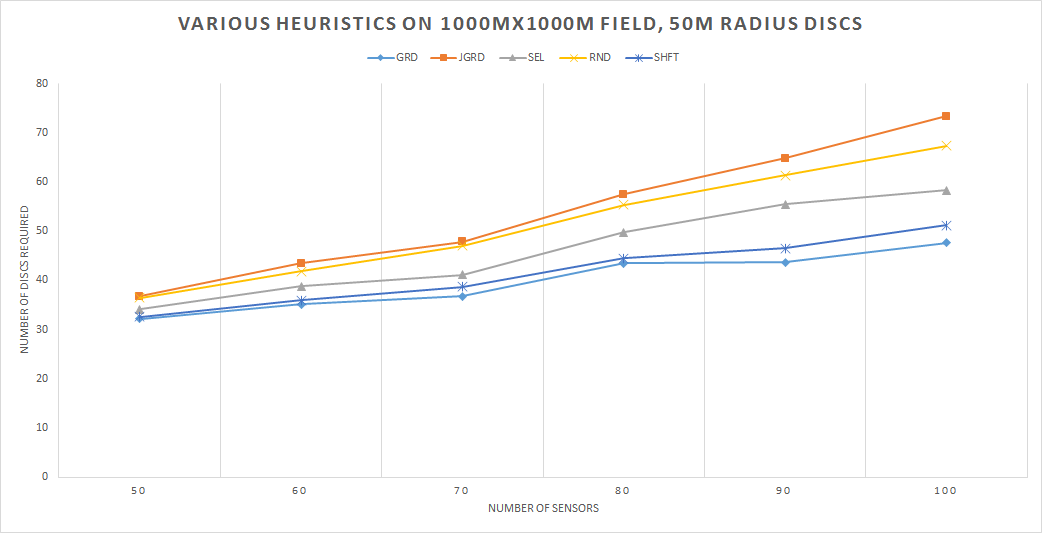
\includegraphics[width=15cm]{discs}
\caption{Results of testing above heuristics and the approximation scheme on a 1000m$\times$1000m field}\label{fig:discResults}
\end{figure}

\section{Euclidean minimum steiner trees}\label{sec:steinerPoints}

\begin{definition}[Euclidean minimum Steiner Tree problem]
Given a set $P$ of points in a 2-D plane as input, the output is a network of line segements connecting all of the points in $S$, with the smallest total (Euclidean) length.
\end{definition}
The line segments making the Steiner Tree need just be incident on the points in $S$. This implies that the algorithm is free to use additional points from the plane, if necessary, to produce the smallest total length network. The additional points are called \emph{Steiner points}

For computing Steiner tress, we use the exact solution finder software GeoSteiner ~\cite{geosteiner1} ~\cite{geosteiner2} ~\cite{geosteiner3}. Following figures show a disc cover of 100 sensors in a 1000m$\times$1000m field with discs of radius 50m, and the Steiner trre of the disc centers thus computed.

\begin{figure}[H]
\centering
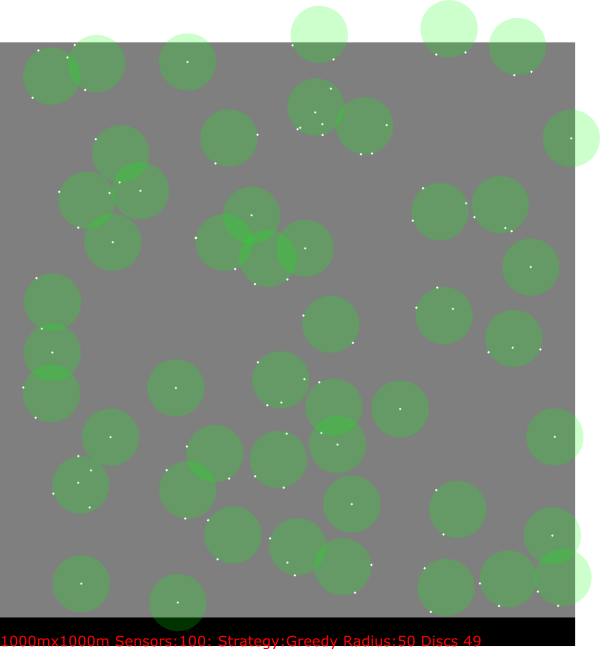
\includegraphics[width=6cm]{figures/disc100.png}
\caption{50m radius disc cover of 100 sensors in 1000x1000 field} \label{fig:disc100}
\medskip
\small
The white dots are sensor positions
\end{figure}

\begin{figure}[H]
\centering
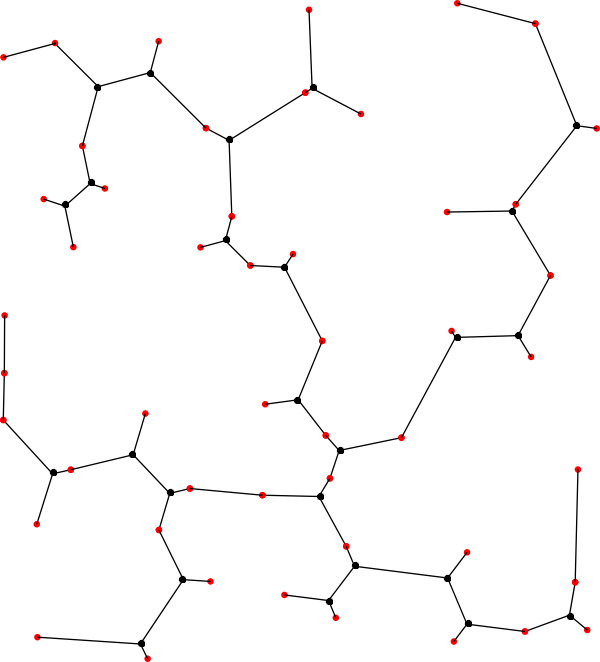
\includegraphics[width=6cm]{figures/steiner100.png}
\caption{The Steiner tree of disc centers of figure \ref{fig:disc100}}
\medskip
\small
The black dots are Steiner points and the red dots are disc centers
\end{figure}
